\documentclass{article}
\usepackage{spconf,amsmath,graphicx,booktabs,url,microtype}
\usepackage[T1]{fontenc}
\setlength{\emergencystretch}{2em}

\title{WHEN DO HAND-CRAFTED EDGES HELP DATA-LIMITED NUCLEUS SEGMENTATION?\\
A CONTROLLED MULTI-SEED AND CROSS-DOMAIN STUDY}
\name{Varun Kumar Dasoju$^{1}$, Qingsu Cheng$^{2}$, Zeyun Yu$^{1}$}
\address{University of Wisconsin--Milwaukee, Milwaukee, WI, USA\\
$^{1}$Department of Computer Science; $^{2}$Department of Biomedical Engineering\\
\texttt{vdasoju@uwm.edu, chengq@uwm.edu, yuz@uwm.edu}}

\begin{document}
\maketitle

\begin{abstract}
Hand-crafted edge channels are often presented as data-efficient priors for nuclear segmentation, yet their gain over matched modern baselines and their behavior under domain shift are rarely isolated. We audit an EfficientNet-B7/UNet++ mammary-nucleus pipeline and conduct 69 matched training runs on the official BBBC039 split. A Gabor-projection-SCSE bundle improves mean test Dice over vanilla B7 by 0.250 percentage points (96.85\% vs. 96.60\%; paired-field bootstrap 95\% CI, 0.197--0.299), but is statistically indistinguishable from a matched UNet++/Xception/SCSE baseline (96.87\%; difference $-0.014$ points, CI $-0.047$--0.018). Validation-only ablations show changes below 0.15 points across orientations, scales, bandwidths, Sobel and sampling, indicating limited parameter sensitivity at this performance level. On 50 TNBC histology images, the unchanged fluorescence-trained vanilla model obtains only 8.07\% patient-macro Dice. A prespecified one-shot polarity correction---grayscale intensity inversion---raises it to 51.30\% (11-patient CI, 36.55--50.15 point gain) without training, but remains below task-specific methods. The study replaces broad superiority claims with reproducible evidence: edge priors offer a small within-screen benefit, while contrast polarity and acquisition domain dominate external transfer.
\end{abstract}
\begin{keywords}
nucleus segmentation, Gabor filters, reproducibility, domain shift, microscopy
\end{keywords}

\section{Introduction}
Accurate nuclear masks support cell counting and quantitative morphology, but annotations are expensive and imaging distributions vary sharply. U-Net~\cite{ronneberger2015unet}, UNet++~\cite{zhou2018unetpp} and pretrained encoders make strong baselines; modern generalist models further raise the comparison standard~\cite{pachitariu2025cellposesam,archit2025microsam}. Consequently, a complex pipeline should be judged against equally trained controls, not historical scores obtained under different splits, budgets or metrics.

This work revisits a project that progressed from 2-D mammary epithelial nuclei to exploratory 3-D reconstruction. Its 2-D method combines a Gabor response, learned input projection, EfficientNet-B7, UNet++ and spatial/channel squeeze-and-excitation (SCSE). Earlier review identified unresolved empty-image scoring, split independence, boundary claims, unequal baselines, Gabor sensitivity, sampling details, statistical uncertainty and absent external validation. We address those issues on public data while restricting the task to \emph{semantic nuclear foreground segmentation}; it is neither breast-cancer diagnosis nor clinical validation.

Our contributions are: (1) a leakage-checked, native-grid and multi-seed evaluation with explicit empty-mask rules and boundary metrics; (2) matched training of six additional architectures and component controls; (3) a test-free, 30-run Gabor/sampling sensitivity analysis; and (4) a complete TNBC transfer stress test showing that polarity mismatch, rather than missing grayscale conversion, explains much of the failure. All attempted configurations and negative results are retained.

\section{Method}
\subsection{Edge-enhanced model}
Let $x$ be percentile-rescaled grayscale intensity. The edge channel is the maximum absolute response of 24 filters (eight orientations and frequencies $f\!\in\!\{0.05,0.15,0.25\}$ cycles/pixel):
\begin{equation}
e(x)=\mathcal N\!\left(\max_{\theta,f}\left|x*\frac{k_{\theta,f}}{\lVert k_{\theta,f}\rVert_1+\epsilon}\right|\right),
\label{eq:gabor}
\end{equation}
where $k$ has size 31, $\sigma=5$, aspect ratio 0.5 and zero phase, and $\mathcal N$ maps to $[0,1]$. L1 normalization replaces unstable signed-sum normalization. A learned $4\!\rightarrow\!16\!\rightarrow\!8\!\rightarrow\!3$ projection feeds ImageNet-pretrained EfficientNet-B7/UNet++/SCSE. Controls remove the edge and SCSE, replace Gabor with Sobel, or use identity-preserving residual fusion
$x_{out}=x_{RGB}+\tanh(a)P([x_{RGB},e])$ with $a_0=0$.

All models minimize $0.5\mathcal L_{Dice}+0.5\mathcal L_{BCE}$. Boundary variants add $0.1\mathcal L_{Dice}(B(p),B(y))$, where $B(u)=\operatorname{maxpool}_3(u)-\operatorname{minpool}_3(u)$. This is an explicit boundary term; no Tversky recall-bias claim is made. Adaptive positive weighting, when audited, safely sets weight one for a zero-positive batch. The sampling ablation uses replacement probability $q_i=w_i/\sum_jw_j$, foreground ratio $r_i$, Canny edge ratio $c_i$, and $s_i=1.5$ if $r_i<0.05$ (otherwise 1):
\begin{equation}
w_i=\begin{cases}0.3,&r_i\le 0.001,\\(2+3r_i)s_i(1+c_i),&r_i>0.001.\end{cases}
\end{equation}

\subsection{Data and leakage controls}
BBBC039v1 contains 200 16-bit $520\!\times\!696$ U2OS Hoechst fields (about 23,000 nuclei) from one chemical screen~\cite{ljosa2012annotated,caicedo2019nucleus}. We use the provider's 100/50/50 train/validation/test split. No crops or ROIs are generated. Identifiers, source groups and decoded-image SHA-256 hashes are checked across partitions. The validation set has 49 foreground fields and one empty field; the test set has no empty references. BBBC039 partly overlaps BBBC038, so BBBC038 is not claimed as independent validation.

TNBC v1.1 provides 50 H\&E images and binary nuclear masks from 11 patients~\cite{naylor2019segmentation}. All images are used exactly once as a post-hoc zero-shot stress test; patient identifiers define inference units. RGB entry and explicit OpenCV grayscale produce bit-identical tensors for all 50 TNBC and 65 BBBC038 images because the pipeline already converts every image to grayscale. Since BBBC039 nuclei are bright on dark backgrounds while H\&E nuclei are dark on bright tissue, we additionally evaluate one fixed transformation, $x'=255-x$, with no fitting, threshold tuning or checkpoint selection. TNBC labels must not be reused to select further preprocessing.

\subsection{Training and statistical analysis}
Every main configuration uses seeds 0/1/2, 20 epochs, $512^2$ inputs, batch size 8, AdamW (learning rate $3\times10^{-4}$, weight decay $10^{-4}$), cosine decay, gradient clipping at 1, and the same flips and $90^\circ$ rotations. The highest complete native-grid validation Dice selects a checkpoint; the final short batch is retained. Threshold 0.5 and no test-time augmentation are fixed for every model. Thus the seven component models (21 runs), ten validation-only sensitivities (30 runs) and six architecture baselines (18 runs) total 69 runs/1,380 epochs.

Predictions are restored to the native grid before Dice, IoU, boundary F1 (BF1) and surface Dice at two pixels, and bidirectional HD95. Both-empty pairs score Dice/IoU/BF1 one and HD95 zero; one-empty pairs score overlap/boundary zero and image-diagonal HD95. Foreground and empty strata are reported separately. For paired comparisons, seed scores are averaged within each field, 10,000 paired bootstrap resamples form 95\% CIs, and two-sided Wilcoxon tests receive Holm correction. TNBC is first averaged within patient. Seed SD quantifies training variation, not biological sample size.

\section{Results}
\begin{table}[t]
\centering\footnotesize
\caption{Matched BBBC039 test results (three-seed mean; Dice includes seed SD). All use the same split and budget.}
\label{tab:main}
\setlength{\tabcolsep}{3.1pt}
\begin{tabular}{@{}lrrrr@{}}\toprule
Model & Params(M) & Dice(\%) & IoU(\%) & BF1(\%)\\\midrule
Vanilla B7 & 68.2 & $96.60\!\pm\!.07$ & 93.44 & 98.53\\
Gabor+projection+SCSE & 68.4 & $\mathbf{96.85\!\pm\!.13}$ & 93.90 & 98.63\\
Gabor+boundary & 68.4 & $96.84\!\pm\!.05$ & 93.88 & 98.68\\
SCSE-only B7 & 68.4 & $96.38\!\pm\!.53$ & 93.06 & 98.48\\
Residual Gabor B7 & 68.4 & $96.57\!\pm\!.27$ & 93.40 & 98.52\\
Residual Sobel B7 & 68.4 & $96.44\!\pm\!.48$ & 93.17 & 98.47\\
Residual Gabor+boundary & 68.4 & $96.61\!\pm\!.31$ & 93.48 & 98.58\\\midrule
U-Net/ResNet-34 & 24.4 & $96.73\!\pm\!.29$ & 93.68 & 98.71\\
U-Net/ResNet-50 & 32.5 & $96.74\!\pm\!.21$ & 93.69 & 98.67\\
UNet++/EfficientNet-B0 & 6.6 & $96.59\!\pm\!.06$ & 93.40 & 98.55\\
UNet++/Xception/SCSE & 35.3 & $\mathbf{96.87\!\pm\!.11}$ & 93.93 & 98.69\\
DeepLabV3+/ResNet-50 & 26.7 & $95.05\!\pm\!.10$ & 90.57 & 96.93\\
FPN/ResNet-50 & 26.1 & $94.97\!\pm\!.28$ & 90.43 & 96.96\\\bottomrule
\end{tabular}
\end{table}

The Gabor bundle gains 0.250 Dice points over vanilla B7 (95\% CI 0.197--0.299; Holm $p=7.34\times10^{-9}$), but has only a $-0.014$ point difference from the strongest matched baseline, UNet++/Xception/SCSE (CI $-0.047$--0.018; Holm $p=.378$). The boundary term and residual fusion do not improve the bundle. Cellpose-SAM obtains 96.95\% semantic Dice as a frozen reference, but unknown pretraining overlap and unequal training make it a contextual comparator rather than a fair baseline.

\begin{figure}[t]
\centering
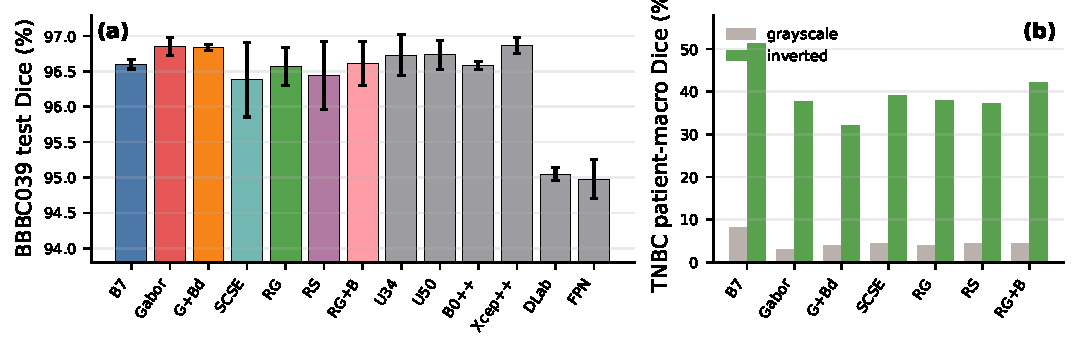
\includegraphics[width=\columnwidth]{figures/submission_results.pdf}
\caption{(a) BBBC039 Dice across all matched models (mean$\pm$seed SD; truncated axis). (b) Patient-macro TNBC transfer before and after fixed grayscale inversion.}
\label{fig:results}
\end{figure}

The validation-only sensitivity study never decodes test cases. Its 8-orientation/3-frequency reference obtains 96.684\% foreground Dice. Four and 12 orientations yield 96.686\% and 96.664\%; one and five frequencies yield 96.723\% and 96.715\%; $\sigma=3$ and 7 yield 96.541\% and 96.709\%; Sobel, neutral-edge and weighted-sampling controls yield 96.727\%, 96.586\% and 96.731\%. Weighted sampling improves foreground Dice by 0.047 points (CI 0.022--0.080) but performs worse on the single empty image, so it is not adopted. These small effects do not support unique optimality of the 24-filter bank.

On TNBC, explicit grayscale exactly reproduces prior results: vanilla B7 is best among the seven configurations at 8.07$\pm$1.39\% patient-macro Dice. Fixed inversion raises vanilla B7 to 51.30$\pm$0.40\%, a 43.24-point patient-paired gain (95\% CI 36.55--50.15; Holm $p=.00684$). The Gabor bundle rises from 2.94\% to 37.66\%. The qualitative example in Fig.~\ref{fig:tnbc} is the median per-image improvement for validation-selected vanilla seed 1, not a best case. Residual over-segmentation confirms that correcting polarity does not solve stain, morphology or tissue-context shift.

\begin{figure}[t]
\centering
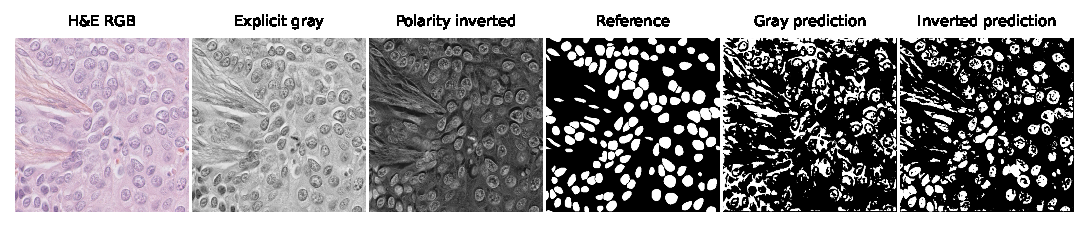
\includegraphics[width=\columnwidth]{figures/tnbc_polarity_example.pdf}
\caption{Actual TNBC image 11\_1: RGB, grayscale, inverted grayscale, reference, and vanilla predictions. Dice increases from 0.212 to 0.655 without retraining.}
\label{fig:tnbc}
\end{figure}

Published BBBC039 values are not directly interchangeable. Caicedo \emph{et al.} report object-level F1 averaged over IoU thresholds (U-Net 0.898)~\cite{caicedo2019evaluation}; SegmentGraph reports pixel Dice 0.9482 and AJI 0.8680~\cite{yi2022segmentgraph}; ASW-Net reports 0.9645 under its DICE1/interior-expansion protocol~\cite{wang2022aswnet}; MA-Net reports 0.973 Dice~\cite{alotaibi2024manet}; and NUSeg reports 0.9693 with fivefold cross-validation and per-epoch test monitoring~\cite{wickramasinghe2024nuseg}. Split, instance postprocessing, selection and metric definitions differ, so none is used for a superiority claim. On TNBC, CellTranspose reports 0.670--0.757 pixel-F1 after 3--10-shot adaptation and Cellpose 0.583 in its selected cross-domain protocol~\cite{he2023celltranspose}; our all-50 zero-shot Dice is descriptive, not a matched leaderboard.

\section{Discussion and conclusion}
The corrected evidence supports a narrow conclusion: hand-crafted edges can yield a small within-acquisition gain over one vanilla B7 control, but architecture choice can match that gain and domain shift overwhelms it. Inversion is a useful diagnostic because it isolates contrast polarity with no learned parameters; its large TNBC effect also exposes the danger of declaring generalization from fluorescence alone.

This study resolves the prior review's computational concerns through public splits, explicit empty handling, equal budgets, SOTA architecture controls, sensitivity ablations, confidence intervals, boundary metrics, complete failures and reproducible code. It does not resolve biological validation. BBBC039 is one U2OS screen, TNBC is post-hoc and label-examined, three seeds are limited, and binary masks do not support touching-instance AP. Foundation-model pretraining overlap remains unresolved. A decisive follow-up should lock polarity normalization on training/validation data, train with patient-separated histology, and evaluate once on an unseen multi-center cohort. Existing 3-D stack results remain preliminary and are not evidence for this 2-D claim.

\clearpage
\section{Compliance with ethical standards}
BBBC039 is an openly released cell-line benchmark. TNBC is previously published, de-identified public histology reused without intervention. \textbf{Before submission, insert the formal UWM IRB/non-human-subjects/exempt determination and identifier here; public licensing alone is not an ethics determination.} No private patient data are analyzed in this paper.

\section{Acknowledgments and disclosures}
This work was supported by U.S. Department of Energy grant DE-SC0025403 \textbf{(authors: confirm)}. The authors declare no competing interests \textbf{(authors: confirm)}. OpenAI Codex assisted with repository auditing, analysis scripts, statistical summaries, figure preparation and language editing. The authors selected the research questions, ran and verified the experiments, inspected all outputs and take responsibility for the manuscript. Figures contain measured data and real images/predictions, not generated microscopy content. Code, manifests and per-image results will be released at \url{https://github.com/vkd14/breast-seg-isbi2027}.

\bibliographystyle{IEEEbib}
\bibliography{references}
\end{document}
